\chapter{Reliable Web Applications}%
\label{cha:reliable_web_applications}

\begin{itemize}
	\item What is the Web?
	\begin{itemize}
		\item What is a Web application?
		\item Rich Internet Application (RIA)?
	\end{itemize}
	\item JavaScript or ECMAScript
	\begin{itemize}
		\item Creation of JavaScript
		\item Browser performance war with Just In Time compilation (JIT)
		\item Explosion of JavaScript and Node
		\item JavaScript issues
		\item The ``transpilation to JavaScript'' paradigm
	\end{itemize}
	\item Frontend Web programming
	\begin{itemize}
		\item Single Page Application (SPA)?
		\item Reactive programming
		\item Functional Reactive programming (FRP)
		\item About the Virtual DOM
		\item Async and the event loop
	\end{itemize}
	\item Elm
	\begin{itemize}
		\item Pure functions
		\item Algebraic Data Types (making impossible states impossible)
		\item Totality
		\item Switch to The Elm Architecture (TEA)
		\item 0 runtime exception
		\item Elm-UI, an alternative layout approach
	\end{itemize}
\end{itemize}


\section{What is the Web?}%
\label{sec:web}

The Internet and the Web are ubiquitous technologies of our everyday lives,
created \comment{around the 80's.}{would be good to be more precise}
Social media, communication, search, news, entertainment, mapping,
shopping, learning, \replace{allmost every}{virtually any} activity is now digital and online.
Simply put, the Web, also called World Wide Web (WWW), consists of the sum of all resources,
available through unique identifiers (URI), that we share on the Internet,
the global network carrying them.

In this chapter, we will recap the Web main evolutions,
from static content to dynamic applications,
and explain the choices we made to build reliable annotation Web applications.

\subsection{What is a Web application?}%
\label{sub:web_application}

An application, in the context of programming (/computers),
is a piece of software presenting information to a user,
usually in an actionable manner.
This includes \replace{things}{programs} like email clients, image \replace{manipulation}{editors}, video games,
word processors, automatic \replace{translation}{translators}, and virtually any functionality
available on a regular computing device.

Web resources are commonly accessible through a Web browser.
Thus, we can define a Web application as a user-facing software,
accessed through a Web browser.
As of May 2019 according to statcounter~\cite{browser-market-share},
the most used Web browsers are Google Chrome (62.7\% of global market share),
Apple Safari (15.9\%) and Mozilla Firefox (5.1\%).

The three pillars of Web applications are HTML, CSS and JavaScript.
HTML, for ``Hypertext Markup Language'' is a description language
organizing a page information as a hierarchy of tagged content.
In Listing~\ref{lst:html}, a ``body'' tag contains three other tags,
a title ``h1'' (h for header), a paragraph ``p'', an image ``img''
and a button not yet linked to any action.
CSS, for ``Cascading Style Sheet'', complements HTML by styling
the content of associated HTML documents.
Listing~\ref{lst:css} shows how \replace{we}{one} would add a left margin of 20 pixels
on all the document body, and make the h1 title red and bold.
\add{Finally, }JavaScript is a scripting language, not affiliated in any form
to the Java programming language.
It is run inside the browser to add dynamic behavior to a Web page.
In Listing~\ref{lst:js} we show how one could count and display
the number of times a user clicked on the button in the page.

\lstinputlisting[language=HTML,caption={Example HTML code.},label={lst:html}]{assets/code/html.html}
\lstinputlisting[language=CSS,caption={Example CSS code.},label={lst:css}]{assets/code/css.css}
\lstinputlisting[language=ES6,caption={Example JavaScript code.},label={lst:js}]{assets/code/js.js}

\subsection{Rich Web Application}%
\label{sub:rich_web_application}

Traditionally, websites used to present their resources in the form of a collection
of static documents, known as Web pages, linked together with hyperlinks.
The nature of Web pages would mostly be informative, visual or textual,
with very few other interactions than navigation through the site by
clicking on the links.

Today, thanks to evolutions of Web technologies that we will detail later,
Web applications have become full-fledged applications with almost
the same capabilities as desktop ones.
They feature functionalities like 3D graphics, \replace{sound}{audio} processing or interactive elements,
and are sometimes called rich web applications.
Similar concepts like ``progressive web applications'' (PWA),
or ``single page applications'' (SPA) are also explained in the following sections.
In the next section, we will dive into the cornerstone of Web pages dynamism, JavaScript.


\section{JavaScript, formally known as ECMAScript}%
\label{sec:javascript_formally_known_as_ecmascript}

\subsection{Genesis of JavaScript}%
\label{sub:genesis_of_javascript}

In 1995, the dominating Web browser was the Netscape Navigator.
Realizing that pages dynamism was key in the \replace{war}{competition} against Microsoft\add{'s}
own Web technologies, Netscape Communications recruited Brendan Eich,
with the aim of integrating a scripting language into their browser.
\replace{And so, in May 1995, he wrote a prototype in 10 days.}{A first prototype was thus developed in 10 days (May 1995).}
Assumably for marketing reasons, it was officially named JavaScript
when released in Netscape Navigator 2.0 beta 3.

Two years later, in June 1997, the European Computer Manufacturers Association
(ECMA) standardized the first version of ``ECMAScript'' as ECMA-262,
JavaScript being its most well\add{-}known implementation.
The ECMAScript (ES) standard has been evolving \add{ever} since.
Today, all browsers fully implement ES5, released in 2009,
and partially implement the most recent versions, ES2015,
ES2016, ES2017 and ES2018.

\subsection{Browser performance war}%
\label{sub:browser_performance_war}

Many browser wars for dominance of market share occurred since the 90's.
\add{In this section, }we are \add{particularly} interested in the JavaScript engine performance war,
starting around 2008 when Google released its Chrome browser.
On September 2, 2008, Google announced a new Web browser called Chrome~\cite{google-chrome}.
Its main selling \replace{point}{feature} was a new JavaScript engine called V8,
greatly improving the browser performances on web applications making
heavy use of JavaScript like their email client \comment{Gmail}{should we notify trademarks with a proper style?}.
\replace{Beware}{Note} that ``performance'' in a browser \replace{is the result of}{depends on} many factors
such that network latency, DOM computation, page rendering or JavaScript processing.
In this section, we will specifically focus \add{on} JavaScript execution performances.

\subsubsection{Dynamic interpretation}%
\label{ssub:dynamic-interpretation}

\replace{Previously, JavaScript was}{JavaScript was originally} an interpreted language.
For each line of code, the engine would translate it into machine code,
and immediately execute it.
This means that for a loop, the \add{same} transformation from JavaScript to machine code
is repeated over and over again.
In addition, JavaScript is a dynamic language, which is \add{both} one of its
strongest points but also a \replace{nightmare for}{huge drag on} execution.
Let's take the function adding two numbers \add{depicted in Listing~\ref{lst:add-js}} as an example
\remove{as in Listing~\ref{lst:add-js}}.

\lstinputlisting[language=JavaScript,caption={Adding two values.},label={lst:add-js}]{assets/code/add.js}

\comment{}{If what follows is a quote, it should be made clearer in the presentation.}
\begin{displayquote}
According to the ECMAScript specification~\cite{ecmascript},
the addition operator either performs string concatenation or numeric addition.
The production ``AdditiveExpression : AdditiveExpression + MultiplicativeExpression''
is evaluated as follows:

\begin{enumerate}
    \item Let lref be the result of evaluating AdditiveExpression.
    \item Let lval be GetValue(lref).
    \item Let rref be the result of evaluating MultiplicativeExpression.
    \item Let rval be GetValue(rref).
    \item Let lprim be ToPrimitive(lval).
    \item Let rprim be ToPrimitive(rval).
    \item If Type(lprim) is String or Type(rprim) is String, then
    \begin{enumerate}
        \item     Return the String that is the result of concatenating ToString(lprim) followed by ToString(rprim)
    \end{enumerate}
    \item Return the result of applying the addition operation to ToNumber(lprim) and ToNumber(rprim). See the Note below 11.6.3.
\end{enumerate}

\textbf{NOTE 1}. No hint is provided in the calls to ToPrimitive in steps 5 and 6. All native ECMAScript objects except Date objects handle the absence of a hint as if the hint Number were given; Date objects handle the absence of a hint as if the hint String were given. Host objects may handle the absence of a hint in some other manner.

\textbf{NOTE 2}. Step 7 differs from step 3 of the comparison algorithm for the relational operators (11.8.5), by using the logical-or operation instead of the logical-and operation.
\end{displayquote}


In theory, if we know that we will only use this function
to sum two numbers, it should compile to a single instruction.
However, due to the dynamic nature of JavaScript,
as specified in the standard, the code has to check if the arguments
are strings, objects, and proceed first with conversions before
eventually reaching the instruction \replace{doing}{that actually computes} the addition.
This process results in one or two orders of magnitude slower code,
compared to statically typed languages like C or Java.

\subsubsection{Just-in-time (JIT) compilation}%
\label{ssub:just_in_time_jit_compilation}

Statically typed languages usually compile code ahead-of-time (AOT),
while dynamically typed languages interpret code at runtime.
Starting with Chrome in 2008, all browser vendors began implementing
just-in-time (JIT) compilers.

The key ingredient is a ``monitor'' sometimes called ``profiler''.
The monitor watches the code while it is run by the interpreter,
and keeps track of how often a piece of code is executed.
Once a path of code is \add{found to be }repeatedly executed, it becomes ``hot'',
which triggers an optimizing compiler.
According to the types previously used in the hot path,
the optimizing compiler will make assumptions enabling
extremely efficient machine code.
If the same code is used once with different types however,
it gets de-optimized back to the baseline compiler.
Multiple optimization and de-optimization round trips
hinders the performances, and consequently will permanently mark
the section as not to be optimized anymore.
For more information on JIT compilation, Lin Clark~\cite{clark-jit}
wrote an \add{enlightning} introductory blog post.

Figure (\alert{TODO faire un schema timeline}) outlines the differences between
interpreting and JITing regarding the ratio of time spent on each phase.
\comment{Fun fact, in V8 the baseline compiler and interpreter is known as ``Ignition''
and the optimizing compiler goes by the name of ``TurboFan''.}{This can probably be ignored :-)}

\comment{}{List of links commented in code}
% December 18, 2007 - https://webkit.org/blog/152/announcing-sunspider-09/
% December 19, 2007 - https://blog.codinghorror.com/the-great-browser-javascript-showdown/
% September 2, 2008 - https://blog.chromium.org/2008/09/google-chromes-need-for-speed_02.html
%  -> release date of Chrome
% September 3, 2008 - https://johnresig.com/blog/javascript-performance-rundown/
% September 3, 2008 - https://arstechnica.com/information-technology/2008/09/new-firefox-javascript-engine-is-faster-than-chromes-v8/
% September 5, 2008 - https://www.zdnet.com/article/is-firefox-faster-than-chrome/
% September 19, 2008 - http://www.satine.org/archives/2008/09/19/squirrelfish-extreme-fastest-javascript-engine-yet/
% November 14, 2008 - https://allanfeid.com/content/javascript-engine-benchmark-test-results
%
% SunSpider: JS perf test suite by WebKit team
% https://www2.webkit.org/perf/sunspider/sunspider.html
% no longer maintained -> cf JetStream
%
% JetStream: Test JS and wasm
% https://browserbench.org/JetStream/
%
% V8 Benchmark: heavy emphasis on recursion


\subsection{Explosion of JavaScript}%
\label{sub:explosion_of_javascript}


\subsubsection{Node.js}%
\label{ssub:node_js}

Not long after the release of the V8 engine from Google,
Ryan Dahl announced at the European JSConf of 2009
a new project named \comment{node.js}{not Node.js ?}~\cite{node-js-speaker}.
As he explains in his talk~\cite{node-js-video},
node is a cross-platform JavaScript runtime environment based on V8.
It features an event-driven architecture, with non-blocking input/output (I/O) APIs.
The project matured from the observation that blocking I/O is extremely non-efficient,
since it requires many threads and \replace{much}{a large} memory to scale with connections.
\remove{JavaScript} Being event-driven by nature in the browser,
\replace{it}{JavaScript} was a perfect fit for the node project.

In order to provide non-blocking asynchronous I/O,
node is composed of an event loop managing callbacks in queued fashion,
and of a thread pool, executing all blocking I/O calls like file reading.
Both are abstracted away by the system, and so a user simply has
to provide callbacks that will automatically be run upon completion of I/O.
An example of reading a file is presented in Listing~\ref{lst:read-file-js}.

\lstinputlisting[%
	language=JavaScript,
	caption={Read a file with node.js.
		Notice the event-driven architecture with an anonymous callback function passed as argument.},
	label={lst:read-file-js}
]{assets/code/readFile.js}


\subsubsection{Node package manager (npm)}%
\label{ssub:node_package_manager_npm_}

\begin{displayquote}
	\textit{``To increase speed, you can either push harder or reduce friction.''}
	--- Isaac Z. Schlueter, node.conf, Portland, OR, May 5th, 2011
\end{displayquote}

With the rise of node for server side JavaScript,
another highly influencial project was born late 2009, npm.
Isaac Z. Schlueter, while working at Yahoo, wanted to increase usage
of JavaScript for full stack web development.
According to him, many people were already pushing hard on node.js,
so he took a stab at lowering friction by creating the Node Package Manager (npm).
The core design choices of npm are rooted in the principle of reducing
most sources of friction, including the following.

\begin{itemize}
	\item \textbf{Conflicting dependencies.}
		When transitive dependencies require different versions of the same package.
		As a consequence, npm retrieves every version needed by dependencies.
	\item \textbf{Inconsistent package installation.}
		Typically, one would need to clone, make, copy, rename files, etc.
		With \verb|npm install|, dependencies are all installed locally,
		under the \verb|node_modules/| directory and usable by invoking
		\verb|require('the-module')|.
	\item \textbf{Publishing difficulties.}
		Usually, package registries require a lot of metadata.
		Npm only requires two fields, name and version.
\end{itemize}

% Mention inspiration from Yahoo's yinst package manager?
% https://www.reddit.com/r/npm/comments/aounfi/best_package_manager/

As a result, npm grew exponentially, to become the world's largest package
registry ever, by a large amount, with over a million packages since June 2019.
At node.conf 2011~\cite{npm-video}, when Isaac Schlueter announced npm 1.0,
the registry contained 1900 packages and almost 800 active package authors.
This roughly corresponds to doubling the registry size every year!

Unfortunately, reduced friction and a policy favoring package creators over users
brought few security issues.
The most notable one is probably the event-stream incident late 2018~\cite{npm-event-stream}
where a new maintainer of the event-stream package added a dependency
to a malicious package, harvesting bitcoin from visitors of a targeted application.
We will discuss later how this risk is reduced with elm packages.


\subsection{JavaScript issues}%
\label{sub:javascript_issues}

\subsubsection{Organic growth and backward compatibility}%
\label{ssub:organic_growth_and_backward_compatibility}

Most programming languages tend to grow in complexity with time.
Regularly, new features are added, and for backward compatibility,
old ways of doing things are kept in the language.
JavaScript is no stranger to this kind of organic growth.
As an example, the language specification of JavaScript is 805 pages~\cite{ecmascript-pdf}.
This is roughly the same size as the Java specification with 772 pages~\cite{java-spec-pdf}
or the C specification with 571 pages~\cite{c-spec-pdf}
To compare, the specification for the Go progamming language
by Google~\cite{go-spec}, contains approximately a 100 pages.

\comment{}{Plus tard mettre citation, it will be finished when there is nothing left to remove.}

The wildest evolutions occurred with ES2015 (previously known as ES6).
Among the confusing ones for beginners are the ``const'' and ``let'' keywords.
They introduce two new ways of declaring variables, bringing it to a total of four,
with the ``var'' keyword and no keyword.
Differences between those are presented in Listing~\ref{lst:var-scope-js}.

\lstinputlisting[language=ES6,caption={Variable scope in JavaScript.},label={lst:var-scope-js}]{assets/code/var-scope.js}

The syntax list continues with ``arrow functions'', ``promises'' and so on.
Most new features are illustrated online at es6-features.org,
I suggest browsing this site for more information.

\comment{}{%
	Il pourrait être aussi intéressant de montionner les choses suivantes :
	- Module systems (CommonJS, AMD, ES2015): https://auth0.com/blog/javascript-module-systems-showdown/
	- ESNext (generators, observers, ...)
}

\subsubsection{Callback hell}%
\label{ssub:callback_hell}

As mentioned when introducing node.js,
JavaScript event-driven APIs rely on callback functions.
Let's consider a simple case where we want to retrieve some data
from a database.
Listing~\ref{lst:callback-hell-sync} outlines how a blocking synchronous API
would look like.
The control flow of the program is easy to follow,
but blocking at ``getDatabase'' and ``db.get'' calls
means the server (or the graphical interface) is non responding
during this time.

\lstinputlisting[%
	language=ES6,
	caption={Hypothetical blocking and synchronous API.},
	label={lst:callback-hell-sync}
]{assets/code/callback-hell-sync.js}

In contrast, the asynchronous callback version
in Listing~\ref{lst:callback-hell-callback},
is efficiently giving back control while waiting for the
database to connect and respond.
The main drawback resides in the complexity of the control flow,
and the verbosity of the code.
By a convention that emerged with time,
callback functions are supposed to handle a potential error
as first argument, and successful result as second argument.
This model continues to bring suffering to JavaScript developers,
and thus has been coined in the community the ``callback hell''~\cite{callback-hell}.

\lstinputlisting[%
	language=ES6,
	caption={Typical asynchronous API based on callbacks.},
	label={lst:callback-hell-callback}
]{assets/code/callback-hell-callback.js}

We should mention that recent JavaScript standards provide new syntax
making use of ``async'' and ``await'' keywords to simplify
the control flow, while preserving the performances of
the callback model.
Listing~\ref{lst:callback-hell-async} shows how the same code can take advantage of the new syntax.
Unfortunately, this is to the detriment of language simplicity,
as explained in the previous point.

\lstinputlisting[%
	language=ES6,
	caption={Asynchronous version with the new async/await syntax.},
	label={lst:callback-hell-async}
]{assets/code/callback-hell-async.js}

\subsubsection{Context of this}%
\label{ssub:context_of_this}

In other object oriented languages,
``this'' (or ``self'') usually refers to the currently used instance of a class.
As defined in the specification,
\textit{The this keyword evaluates to the value of the ThisBinding of the current execution context.}
JavaScript not being a typical object oriented language,
``this'' can take many shapes, depending on the execution context.
The execution contexts are in a stack where new contexts are created and pushed
whenever code not associated with the current context starts running.
This typically happens in function calls.
Let's take Listing~\ref{lst:this-js} to exhibit some odities of the ``this'' value.

\lstinputlisting[%
	language=ES6,
	caption={Value of ``this'' in JavaScript.},
	label={lst:this-js}
]{assets/code/this.js}

By default, if ``this'' is undefined, as in lines 17 and 18,
it is binded to the global object.
At line 11, we define ``x = 1'' with no keyword,
so ``x'' is a global variable.
As a result, line 17 and 18 print 1.
The definitions of the ``log'' and ``logF'' methods on the ``Who'' class
lines 7 and 8 are equivalent. The behavior of ``this'' in that context,
is what we expect to see for methods call on objects and thus,
lines 20 and 21 both print 2.
The ``call'' function (and some others), used for the definition of the ``logCall'' method,
enables binding of the ``this'' value to a specific object given as first argument.
That is why line 23 prints 3.

Now the most surprising results are lines 19 and 22, both printing 1 instead of 2.
At line 13, ``logMe'' is defined as the same function than ``me.log'' which
actually is the original ``log'' function.
As a consequence, line 19 is strictly equivalent to line 18, and they both print 1.
Finally, the ``logF2'' method also prints 1 because it's definition isn't the log function
(as defined for the ``log'' method) but rather calls the ``log'' function which
generates another context in which ``this'' is not defined anymore.
The behavior is thus the same than for lines 17 and 18, which binds ``this'' to the global object,
and prints the global variable ``x = 1''.

\subsubsection{Dynamic typing and implicit conversions}%
\label{ssub:dynamic_typing_and_implicit_conversions}

JavaScript is dynamically typed language.
This means that types of values are only known at runtime,
and that they can change during the execution of the program
as shown in Listing~\ref{lst:dynamic-js}.

\lstinputlisting[%
	language=ES6,
	caption={Dynamic typing in JavaScript.},
	label={lst:dynamic-js}
]{assets/code/dynamic.js}

In addition, JavaScript performs implicit conversions between type,
depending on the operators and functions being used.
In Listing~\ref{lst:weak-js}, the number 42 gets converted into the string ``42''
before concatenation, and the string ``6'' is converted to the number 6
before multiplication with the number 7.

\lstinputlisting[%
	language=ES6,
	caption={Weak typing in JavaScript (implicit conversion).},
	label={lst:weak-js}
]{assets/code/weak.js}

By combining dynamic types, and implicit conversions,
JavaScript often generates extremely surprising situations,
resulting in unexpected behaviors.
It can also lead to very original use cases.
In 2010, an informal code obfuscation competition resulted in the creation
of a subset of JavaScript containing only six characters~\cite{jsfuck},
``['', ``]'', ``('', ``)'', ``!'' and ``+'',
able to represent any valid JavaScript code.
The value ``false'' would be obtained with ``![]'',
since negation of an empty array returns ``false'' according to JavaScript specification.
Numbers, characters, and other language constructs are obtained through similar
implicit conversion tricks.

\subsubsection{Undefined is not a function}%
\label{ssub:undefined_is_not_a_function}

\begin{figure}[ht]
	\centering
	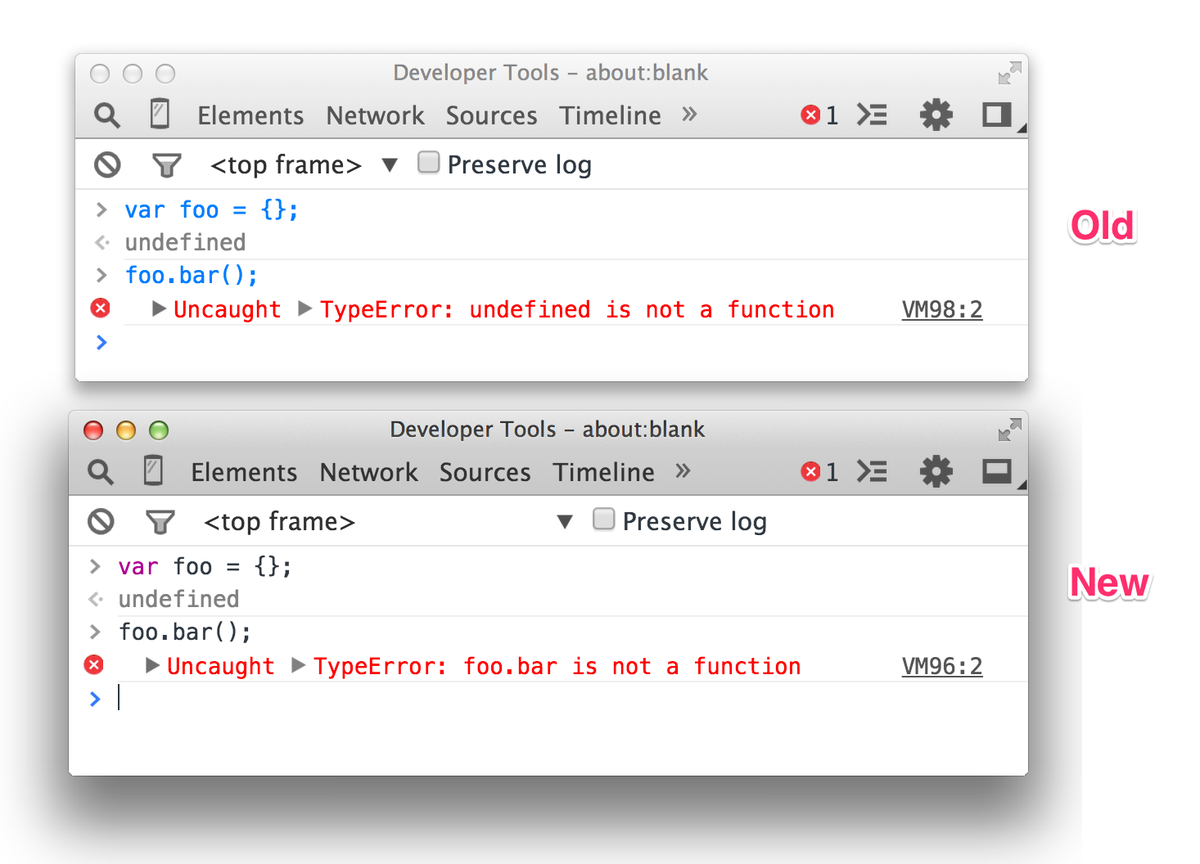
\includegraphics[width=1.0\linewidth]{assets/img/undefined-improved.png}
	\caption{Tweet by Addy Osmani (21-Feb-2015) announcing error report improvements in Chrome.}%
	\label{fig:undefined-improved}
\end{figure}

For JavaScript developers previous to 2015,
the error ``undefined is not a function'' was famous for not being helpful.
This error would very often rise from a typo somewhere in the code.
Due to the dynamic nature of JavaScript, the error can be reported late in the call stack.
Indeed, even if an error in the code might create an ``undefined'' value,
it is only later when called, that an uncaught error would trigger.
As shown in Figure~\ref{fig:undefined-improved}, browsers are more helpful now,
at the cost of loosing an iconic error for all JavaScript developers.
Yet not having a compile step prevents advanced static analysis of the code,
and at the same time lengthen the feedback loop to fix errors.


\subsection{JavaScript as a compilation target}%
\label{sub:javascript_as_a_compilation_target}

As we now know, JavaScript exists since 1995, and from 1997 onward,
has mostly been the only way to run code dynamically in the browser.
For this reason, many alternative languages started to treat JavaScript
as a compilation target to run code in a browser.

\subsubsection{Multi-tier programming}%
\label{ssub:multitier}

Haxe was probably the first production ready language to target JavaScript, in 2006.
At this time, there was no JIT, and JavaScript performances weren't great either.
Yet some people where trying to make the web a video and gaming platform.
Flash, a multimedia platform running the ActionScript language was the rising star at this time.
In 2005, YouTube made use of a Flash player to distribute videos.
Haxe, created by Nicolas Cannasse~\cite{haxe-interview},
had a clear purpose, remove the overhead of composing many languages like a Flash client,
a Web server, and additional JavaScript glue when designing Web games.

Many other languages followed that trend of using the same language
for server and client code, sometimes called ``isomorphic'' frameworks.
Google announced their Google Web Toolkit (GWT) in May 2006~\cite{gwt},
enabling Java developers to build client application.
The Ocsigen framework by V. Balat et al.~\cite{balat2006ocsigen} in 2006
enabled fully featured applications in the OCaml programming language.
The Opal compiler~\cite{opalrb} transforms ruby code into JavaScript,
enabling full stack Ruby with the rails framework for the backend.
Today, most programming languages can target JavaScript,
including Python, C, Erlang, Haskell, etc.

Around the same period, academic research is also trying to solve
what we call multi-tier web programming with unique new languages like Links
by E. Cooper et al.~\cite{cooper2006links},
or Hop by Serrano et al.~\cite{serrano2006hop} in 2006.
Those efforts are continuing with for example
A. Chlipala et al.~\cite{chlipala2015ur} who created the Ur/Web variant
of the Ur modelling language,
or Sinha et al.~\cite{sinha2015simplifying} with the WebNat programming language in 2015.
Unfortunately, those research attempts at novel ways of programming the Web
are not adopted by the programmers.
According to~\cite{sinha2015simplifying},
one of the key factors is that experienced Web programmers want fine grained
control on the generated code for designing complex applications.

\subsubsection{JavaScript as the main target}%
\label{ssub:javascript_as_the_main_target}

Instead of trying to tackle both server and client programming,
a new category of languages emerged focused on the client side,
with JavaScript being the only, or main compilation target.
The most notable ones are CoffeeScript~\cite{coffeescript} released in 2009
by Jeremy Ashkenas, Dart~\cite{dart-blog} designed by Lars Bak
(creator of the V8 engine) and Kasper Lund for Google in 2010,
Elm~\cite{czaplicki2013asynchronous} the product of Evan Czaplicki senior thesis
on functional reactive programming in 2012,
and Reason~\cite{reason} (also known as ReasonML) in 2016 by Jordan Walke,
also the original designer of the React framework we will discuss later.

One can notice that appart from Dart, which is heavily object oriented,
most attempts at new programming languages for the client follow the functional paradigm.
It is not estranged from guaranties brought by
functional programming that we will develop when exploring the Elm programming language.

A note about the Dart language, it has been abandonned for Web programming,
but found a new home in the Flutter framework~\cite{flutter}, released in 2017,
targeting mainly native development of mobile applications on iOS and Android.

\subsubsection{Gradually typed JavaScript}%
\label{ssub:gradually_typed_javascript}

Coding with a completely different language is a rather extreme approach
which can feel overwhelming.
From this observation, both Microsoft and Facebook decided to bring
new contributions to the JavaScript ecosystem in the form of gradual typing.
Gradual typing is a type system where values are partially typed.
Some may be typed, and consequently static typing rules are verified,
and some may be untyped, left for compile-time verifications.

In October 2012, Microsoft released TypeScript~\cite{bierman2014understanding},
a superset of JavaScript, enabling type annotations.
As a consequence, any valid JavaScript program is also a valid TypeScript program.
This property was most certainly the major success factor of TypeScript.
Programs can be ported progressively to benefit from static analysis.
Listing~\ref{lst:add-ts} exhibits the core type annotation feature of TypeScript.

\lstinputlisting[%
	language=JavaScript,
	caption={JavaScript and TypeScript version of an add function.},
	label={lst:add-ts}
]{assets/code/add.ts}

Another benefit of static typing that JavaScript developers are discovering when
switching to TypeScript is the improved IDE support,
with better autocompletion tools, jumping to definitions and other support from your editor.

In 2014, another tool named Flow and led by Facebook~\cite{chaudhuri2017fast}
enabled gradual typing of JavaScript.
Ultimately, TypeScript seems to have taken the biggest part of the cake,
but choosing between the two will most likely depend on how well they integrate
with your working framework.

\subsubsection{JavaScript transpilation}%
\label{ssub:javascript_transpilation}

Despite increasing language complexity
as explained in Section~\ref{ssub:organic_growth_and_backward_compatibility},
ES2015 and later specifications brought very appreciated features to the table,
many influenced by other languages like CoffeeScript.
The ``async / await'' pair of keywords is such example of syntax
improving on complexity of the code control flow.
New specifications however, are not always immediately available in all browsers,
especially mobile versions.
But there is one version of JavaScript fully supported on all browsers, ES5.
Inspired by the traceur tool by Google engineers,
Sebastian McKenzie jumped head first into writing 6to5~\cite{babel}
on September 2014, at the age of 17.
His 6to5 project, now renamed Babel, is known as a JavaScript ``transpiler'',
i.e.\ a program converting recent JavaScript source code into another (older) version
of JavaScript source code.
Today, Babel has become one of the most used tools
with 7 million weekly downloads on npm.


\section{Frontend Web programming}%
\label{sec:frontend_web_programming}


\subsection{Single Page Application (SPA)}%
\label{sub:single_page_application_spa_}

Angular, React, Vue

\subsection{Functional reactive programming}%
\label{sub:functional_reactive_programming}

Elm, FRP research papers.

\subsection{Virtual DOM}%
\label{sub:virtual_dom}

Why modifying the DOM directly is a mistake.
Understanding the animation frame loop.

\subsection{Assets compilation}%
\label{sub:assets_compilation}

How JavaScript switched from a human readable interpreted file,
to a modularized, transpiled, minified, gzipped compilation target.

\section{Elm}%
\label{sec:elm}

\subsection{Pure functions}%
\label{sub:pure_functions}

And referential transparency.

\subsection{Algebraic Data Types (ADT)}%
\label{sub:algebraic_data_types_adt_}

Sum and product types, ``custom'' types as they are called in Elm.
Analogy between types and cardinality of sets.

\subsection{Total functions}%
\label{sub:total_functions}

0 runtime exception.
Enjoyable refactoring.
The compiler is your assistant.

\subsection{The Elm Architecture (TEA)}%
\label{sub:the_elm_architecture_tea_}

An inspiration for Redux.

\subsection{Elm-UI, an alternative layout strategy}%
\label{sub:elm_ui_an_alternative_layout_strategy}

When your layout compiles it is correct.
